\section{G2: 2D reconstruction of the horizontal plane}
In the following section we are going to explore several ways to obtain a metric rectification of the original image.

In order to establish which are the possible and navigable ways to compute the metric rectification of our original image, we list the detected object in our image that could help us to achieve our objective:
\begin{itemize}
    \item 3 independent families of orthogonal lines: $l_i$, $m_j$ and $h_k$ lines; we know they are orthogonal each other since they represents the three axis in the original \verb|3D| scene
    \item the horizontal circumference $C$
    \item the unknown planar curve $S$
\end{itemize}

\bigbreak

Based on the available objects, we can compute the desired metric rectification using two different methods:
\begin{itemize}
    \item metric-stratified method
    \item metric rectification using one circle
\end{itemize}

We can't use the method involving 5 pairs of orthogonal lines, because we haven't the necessary pairs of independent orthogonal lines; we have only 3, as reported previously.

\subsection{Metric stratified method}
The metric stratified method consists of first performing an affine rectification and then finding $C_{\infty}^{*'}$ through two more constraints.
\subsubsection{Affine rectification}
By selecting two independent pairs of parallel lines in the original image scene, we can estimate their intersection using the cross product. This allows us to determine the image of the line at infinity that connects the resulting vanishing points.

The goal of affine rectification is to map the image of the line at infinity to its canonical position, thereby preserving and restoring the parallelism of lines. This is a direct result of aligning the line at infinity with its original position.

Since our objective is to compute a 2D reconstruction of the horizontal plane, the lines to be selected are $l_i$ and $m_j$, for which we have already computed $l_{\infty}'$ in the previous section (\ref{infLine}).

The computed affine-homography matrix is the following:
\[
    H_{aff}
    =
    \begin{bmatrix}
        1.0000 & 0 & 0 \\
        0 & 1.0000 & 0 \\
        -0.0001 & -0.0011 & 1.0000
    \end{bmatrix}
\]

The affine rectified image is shown below:
\begin{figure}[H]
    \centering
    \includegraphics[width=0.75\linewidth]{img/affineRectifiedImage.jpg}
    \caption{Affine rectified image}
    \label{fig:affineRectification}
\end{figure}

\subsubsection{Metric rectification using imaged right angles}
After obtaining the affine rectified image, two additional constraints are necessary to address the two degrees of freedom associated with the circular points. These constraints allow the computation of a metric rectification, which restores the metric properties of the world plane.

One approach to derive these constraints is by identifying two imaged right angles on the world plane. In the affine rectified image, let $l'$ and $m'$ represent an orthogonal line pair $l$ and $m$ on the world plane. The orthogonality condition can then be leveraged, where the cosine of the angle between two lines is given by:

\begin{equation}
    \cos\theta = \frac{l^{'T} C_\infty^{*'} m^{'}}{\sqrt{(l^{'T} C_\infty^{*'} l^{'}) (m^{'T} C_\infty^{*'} m^{'})}} \label{eq:1}
\end{equation}

Since $l$ and $m$ are orthogonal, $\cos \theta = 0$, which simplifies to:

\[
    l^{'T} C_\infty^{*'} m^{'} = 0
\]

By substituting the definition of $C_\infty^{*'}$, the constraint becomes:

\[
    (l'_1 \quad l'_2 \quad l'_3)
    \begin{bmatrix}
        KK^T & 0 \\
        0^T & 0
    \end{bmatrix}
    \begin{pmatrix}
        m'_1 \\
        m'_2 \\
        m'_3
    \end{pmatrix}
    = 0
\]

This equation establishes the necessary relationship to constrain the circular points and achieve metric rectification.

Despite selecting two independent pairs of orthogonal lines, as illustrated in the following image, we were unable to compute the rectified image due to likely numerical errors.


\begin{figure}[H]
    \centering
    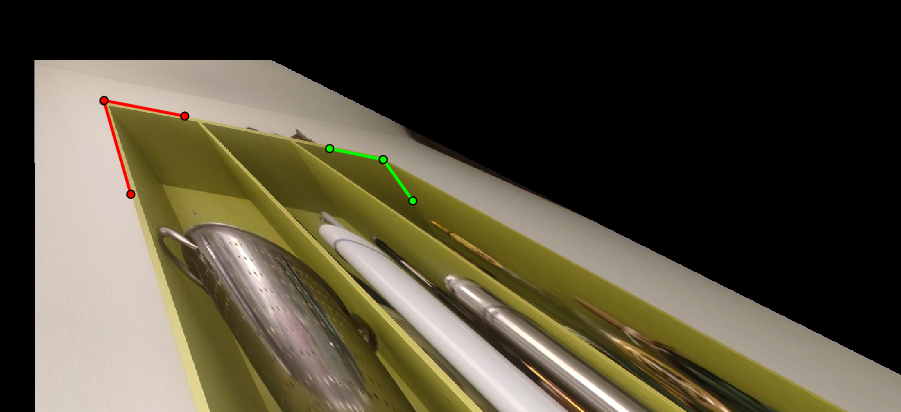
\includegraphics[width=0.75\linewidth]{img/G2/tryMetric.jpg}
    \caption{Two independent pairs of orthogonal lines}
    \label{fig:twoPairsOfOrthogonalLines}
\end{figure}

In conclusion, a different approach must be adopted to achieve the metric rectification of the provided image.

\subsection{Metric rectification using one circle}
Having detected the circumference $C$ in section (\ref{sec:detectedC}), we can use this information to compute the metric rectification.

The image of the circular points is determined by the intersection of the conic $C$ and the line at infinity $l_\infty'$. This intersection corresponds to the points on the conic that lie at infinity in the projective plane.

\paragraph{Conic equation} A general conic in homogeneous coordinates $[x, y, 1]^T$ is represented as:
$$C(x,y) = ax^2 + bxy + cy^2 + dx + ey + f = 0$$
Where $C$ if the conic matrix:
\[
    C
    =
    \begin{bmatrix}
        a & b/2 & d/2 \\
        b/2 & c & e/2 \\
        d/2 & e/2 & f
    \end{bmatrix}
    = 
     \begin{bmatrix}
        -3.20 \times 10^{-7} & \frac{2.12 \times 10^{-7}}{2} & \frac{2.53 \times 10^{-4}}{2} \\
        \frac{2.12 \times 10^{-7}}{2} & -3.06 \times 10^{-6} & \frac{3.32 \times 10^{-3}}{2} \\
        \frac{2.53 \times 10^{-4}}{2} & \frac{3.32 \times 10^{-3}}{2} & -1.00
    \end{bmatrix}
\]

\paragraph{Line at infinity} The line at infinity $l'_\infty$ in homogeneous coordinates is expressed as:
$$l'_\infty(x, y) = l_1x + l_2y + l_3 = 0$$

\paragraph{System of equations}
The intersection of the conic and the line at infinity is obtained by solving the following system of equations:
\begin{itemize}
    \item Conic equation:
    $$ax^2 + bxy + cy^2 + dx + ey + f = 0$$
    \item Line at infinity:
    $$l_1x + l_2y + l_3 = 0$$
\end{itemize}

\paragraph{Circular points in homogeneous coordinates} The resulting points in homogeneous coordinates are:
\[
    s_1 = \begin{bmatrix}
        x_1 \\
        y_1 \\
        1
    \end{bmatrix}, \quad
    s_2 = \begin{bmatrix}
        x_2 \\
        y_2 \\
        1
    \end{bmatrix}
\]
These points correspond to the \textbf{image of the circular points}.

The computed circular points are complex conjugates, as they lie on the real conic and at infinity. Their representation enables constructing the \textbf{dual conic of the circular points}:

$$C_\infty' = s_1s_2^T + s_2s_1^T$$

The final metric rectification matrix $H_{met}$ obtained is:
\[
    \label{metricRectMatrix}
    H_{met}
    =
    \begin{bmatrix}
        1.4243 & -6.9489 \times 10^{-1} & 0 \\
        -6.9489 \times 10^{-1} & 2.1380 & 0 \\
        -1.0000 \times 10^{-4} & -1.1000 \times 10^{-3} & 1
    \end{bmatrix}
\]

and the final metric rectified image is:
\begin{figure}[H]
    \centering
    \includegraphics[width=0.75\linewidth]{img/G2/metric_rectified_image.jpg}
    \caption{Metric rectified image using $C$}
    \label{fig:metricRectificationUsingOneCircle}
\end{figure}

\subsection[Estimation of \textit{m} Lines]{Estimation of $m$}\label{estimationDepth}
To compute the depth $m$ of the parallelepiped, we start by considering its known length $l = 1 \, m$. Using the lines \textit{l} and the hypotenuse of the triangle and the angle $\alpha$ between them (refer to the accompanying illustrations for clarity), we calculate $\cos\alpha$ using equation \ref{eq:1}.

From the metric rectified image, we observe that $l$ and $m$ are orthogonal, forming a right triangle. According to the properties of a right triangle, the depth $m$ can be expressed as:

$$ m = l \sin\alpha$$

Given $\cos\alpha$, we compute $\sin\alpha$ using the trigonometry identity:
$$\sin\alpha =  \sqrt{1-\cos^2\alpha}$$

Substituting the calculated values, we find:
$$m \approx \frac{1}{3} \, m$$

\begin{figure}[H]
    \centering
    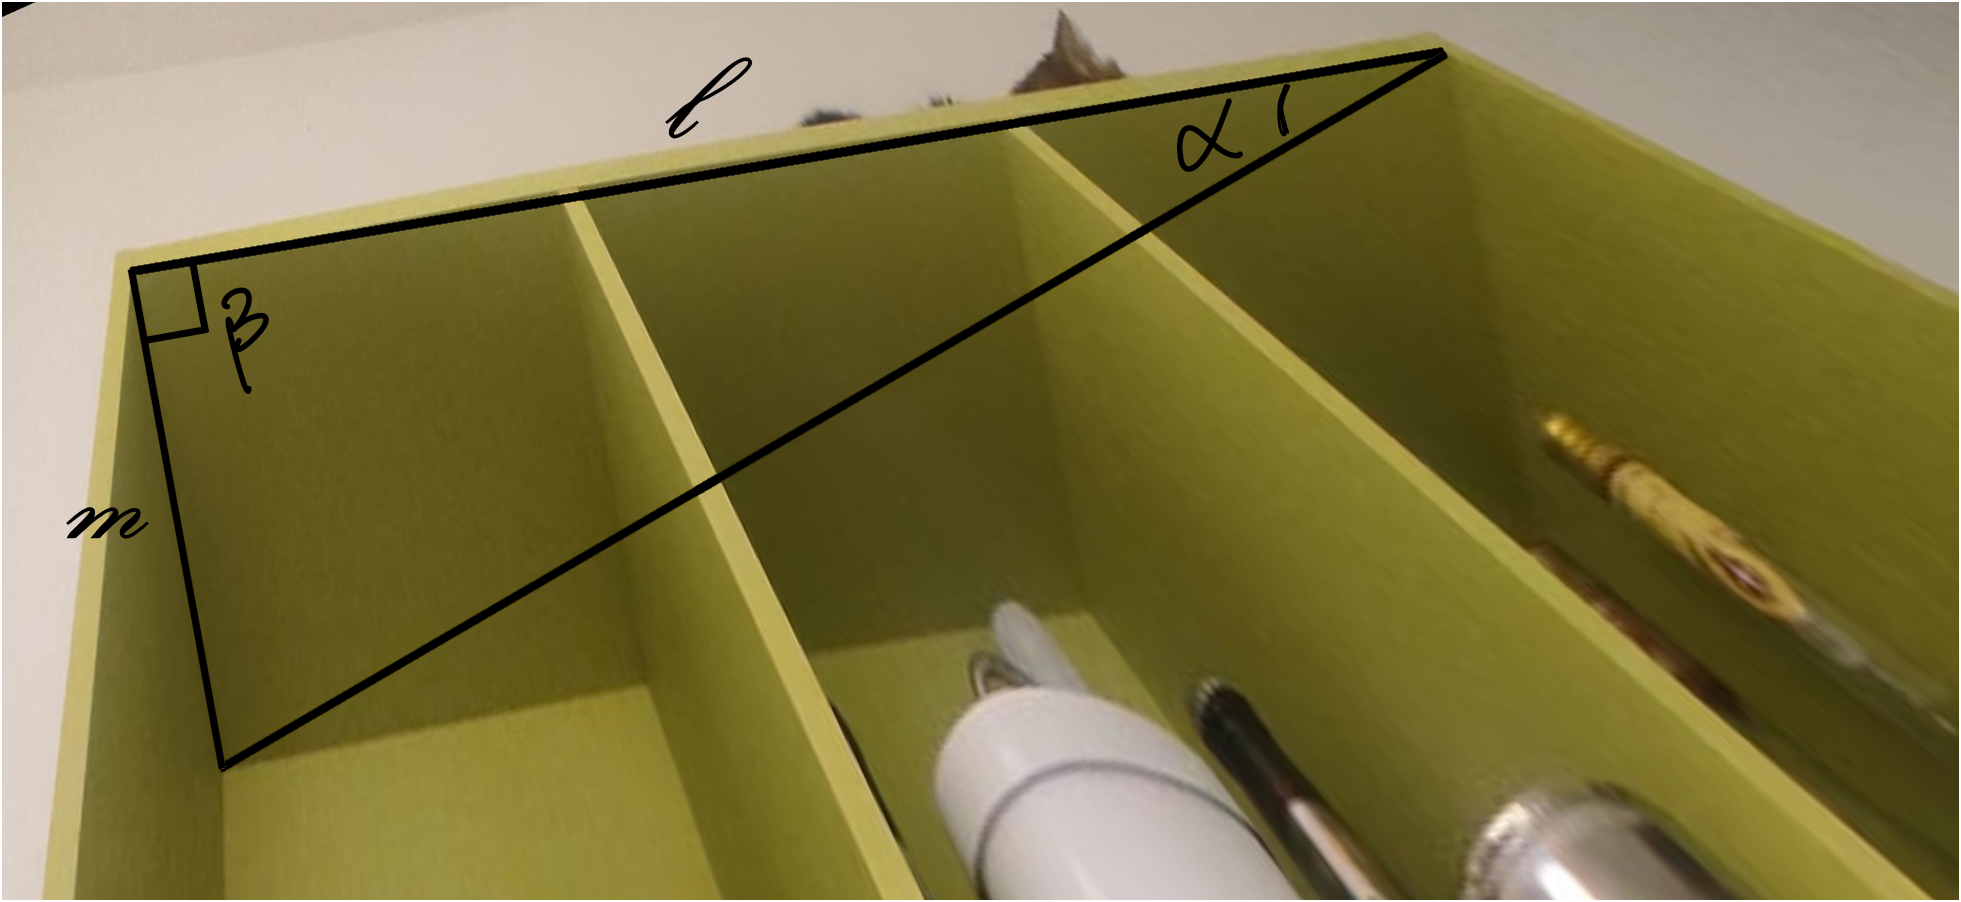
\includegraphics[width=0.7\linewidth]{img/triangleWithAngles.png}
    \caption{Triangle in metric rectified image}
    \label{fig:triangleWithAngles}
\end{figure}

\subsubsection{Double check of the result}
To double check the obtained result, we start doing an hypothesis: the parallelepiped is divide into three parts of equals length.
\paragraph{Compute cross ratio}
To prove it, we need to compute the cross ratio (\textit{CR}) of every divisor, between points $A$, $B$, $C$, $D$ shown in the following image.

\begin{figure}[H]
    \centering
    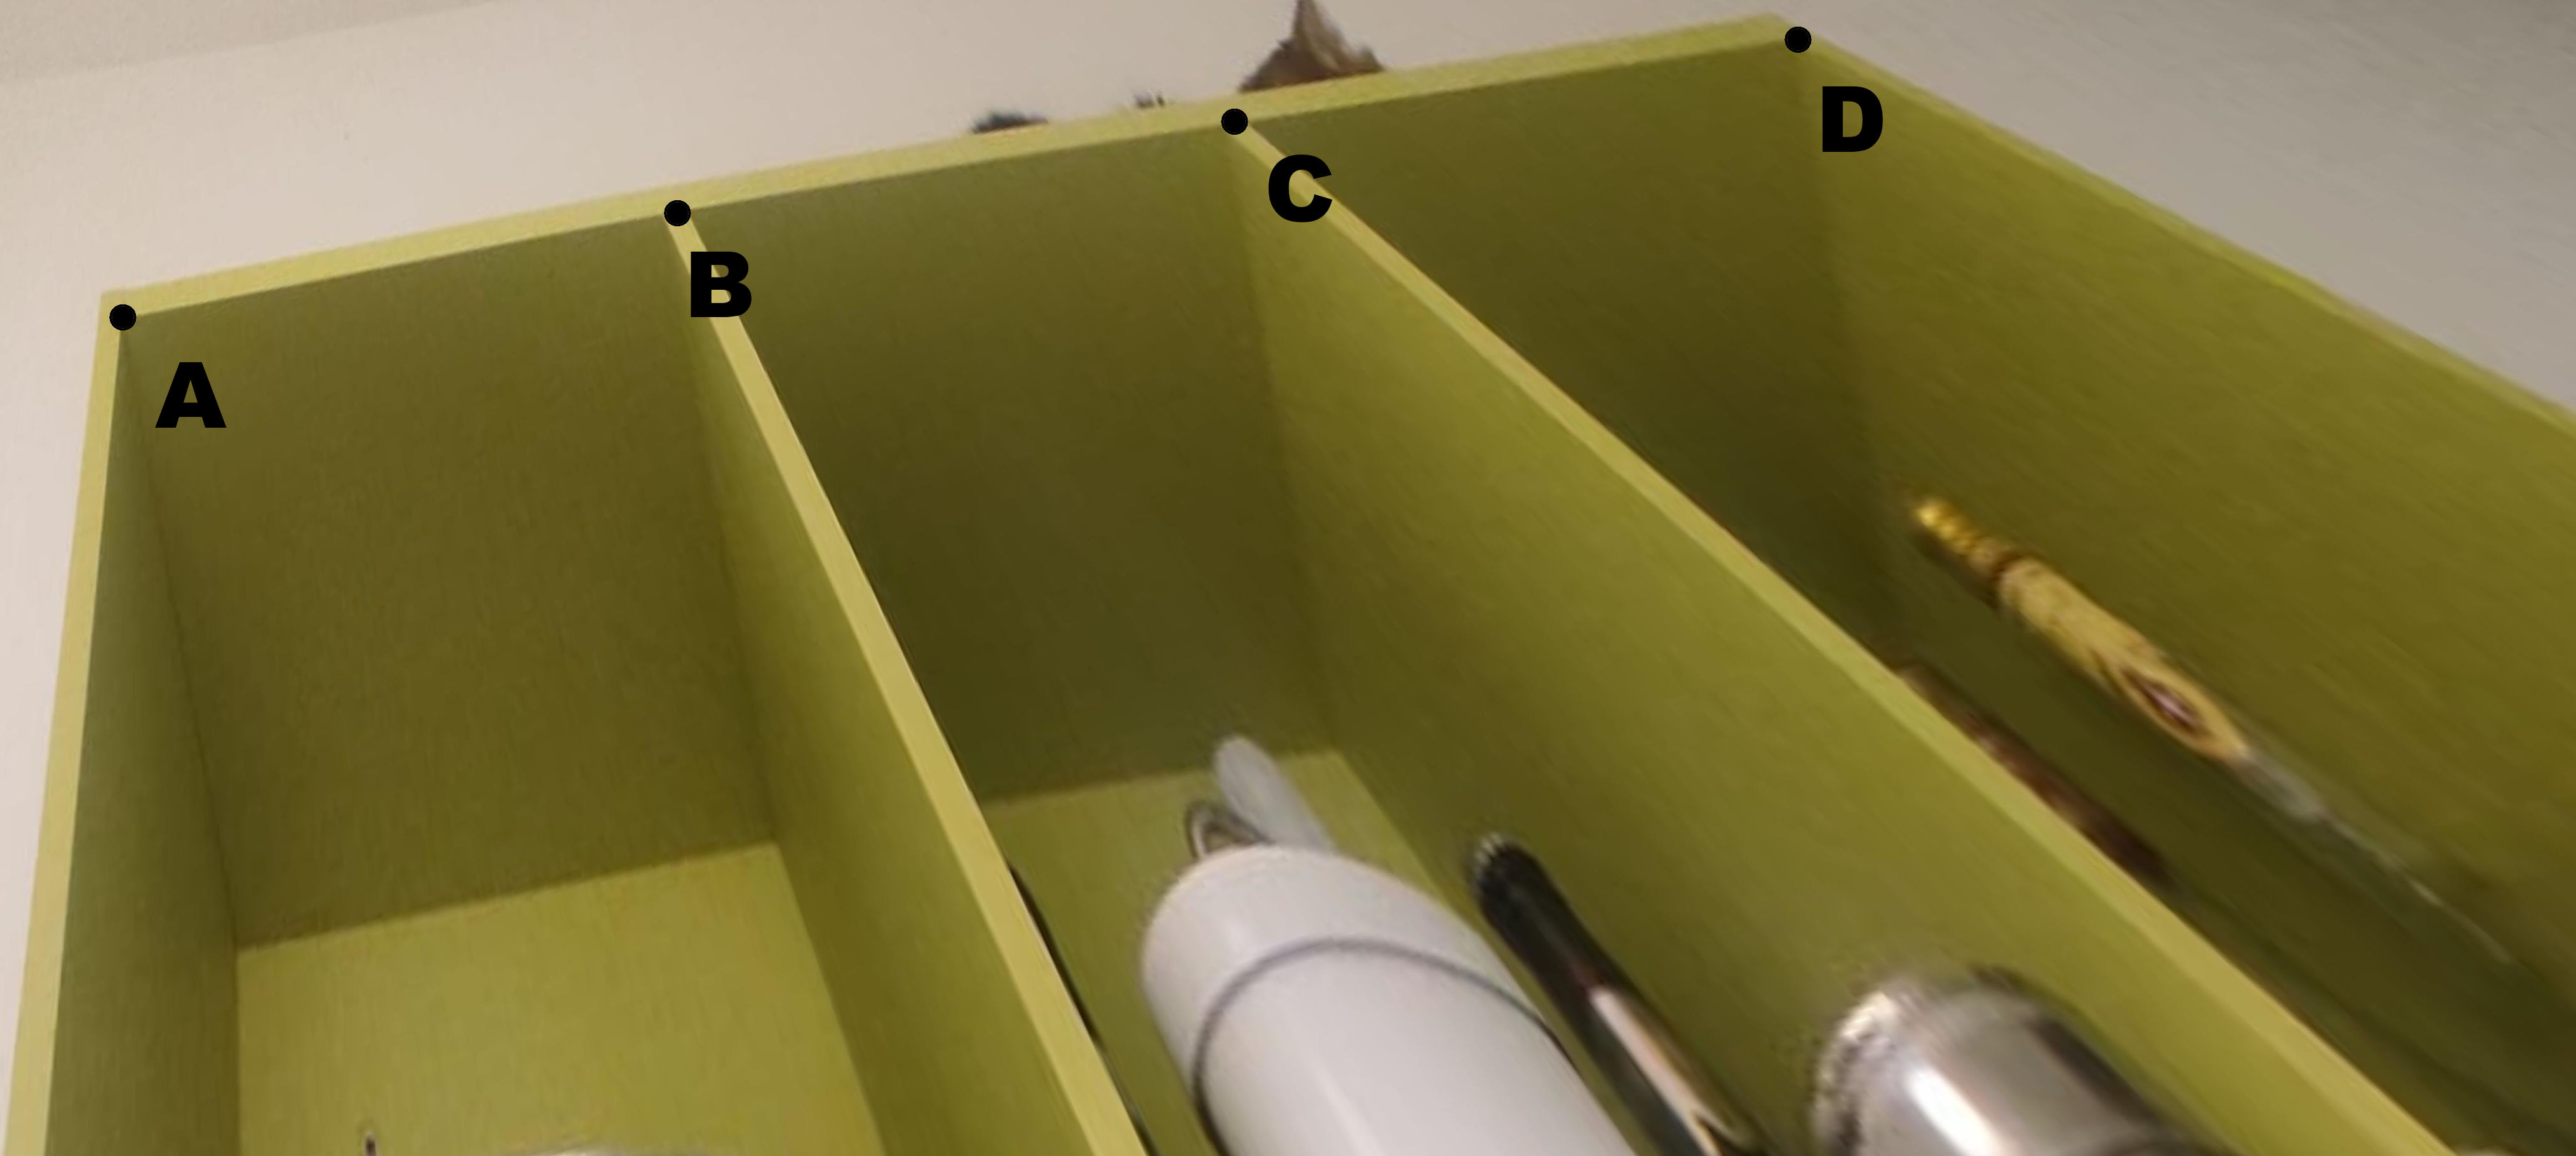
\includegraphics[width=0.7\linewidth]{img/cr.png}
    \caption{Selected points to compute $CR$}
    \label{fig:selectedPoints}
\end{figure}

In real world, based on our hypothesis we know:
\begin{itemize}
    \item $A = 0 \, m$
    \item $B = \frac{1}{3} \, n$
    \item $C = \frac{2}{3}\, m$
    \item $D = 1 \, m$
\end{itemize}

Remembering the cross ratio of a 4-tuple of collinear points formula:
$$ CR_{Y,Z,X_1,X_2} = \frac{c-a}{c-b} / \frac{d-a}{d-b}$$
\begin{figure}[H]
    \centering
    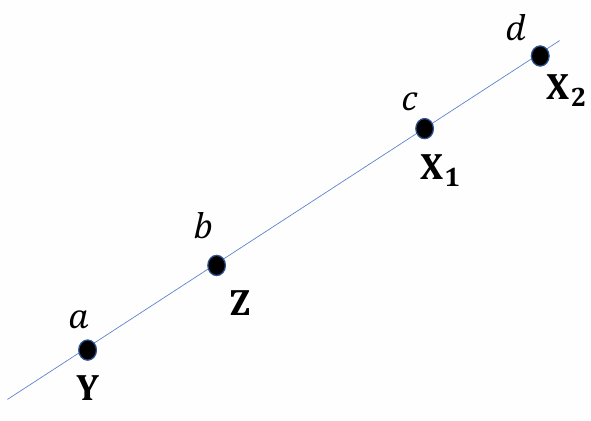
\includegraphics[width=0.5\linewidth]{img/crTheory.png}
    \caption{Cross ratio formula}
    \label{fig:crTheory}
\end{figure}

The real-world aspect ratio is computed as:

$$CR_{real} = \frac{\frac{2}{3} - 0}{\frac{2}{3} - \frac{1}{3}} / \frac{1 - 0}{1 - \frac{1}{3}} = \frac{4}{3}$$

By executing the code available in \verb|G2\cr.m|, which involves manually selecting and obtaining the pixel coordinates of the points shown in Figure \ref{fig:selectedPoints}, the image aspect ratio was determined to be:

$$CR_{image} = 1.3484 \approx \frac{4}{3}$$

Since the aspect ratio ($CR$) is preserved from the real world to the image and the computed ratios are approximately equal, we can conclude that the parallelepiped is divided into three blocks of equal length.

\paragraph{Estimation of $m$}
From the following image, which is a zoom of the metric rectified image, we can see:
\begin{itemize}
    \item lines $l_x$ and $l_y$ are parallel, as direct consequence of metric rectification, since parallel lines in the real world remain parallel in the metric rectified image 
    \item lines $m_1$ and $m_2$ are parallel, for the same reason above
    \item lines $m_1$ and $l_x$ are orthogonal, as direct consequence of the metric rectification computed
    \item lines $m_1$ and $l_y$ are orthogonal, since $m_1$ is orthogonal to $l_x$ and $l_x$ is parallel to $l_y$ 
\end{itemize}
\label{square}
So, we can clearly see that all the internal angles are right angles and we can hypothesize that the figure is a square. To confirm our hypothesis, we just measure the angle between between the intersection of the two diagonals and check if is a square one, again using the formula \ref{eq:1}.

\begin{figure}[H]
    \centering
    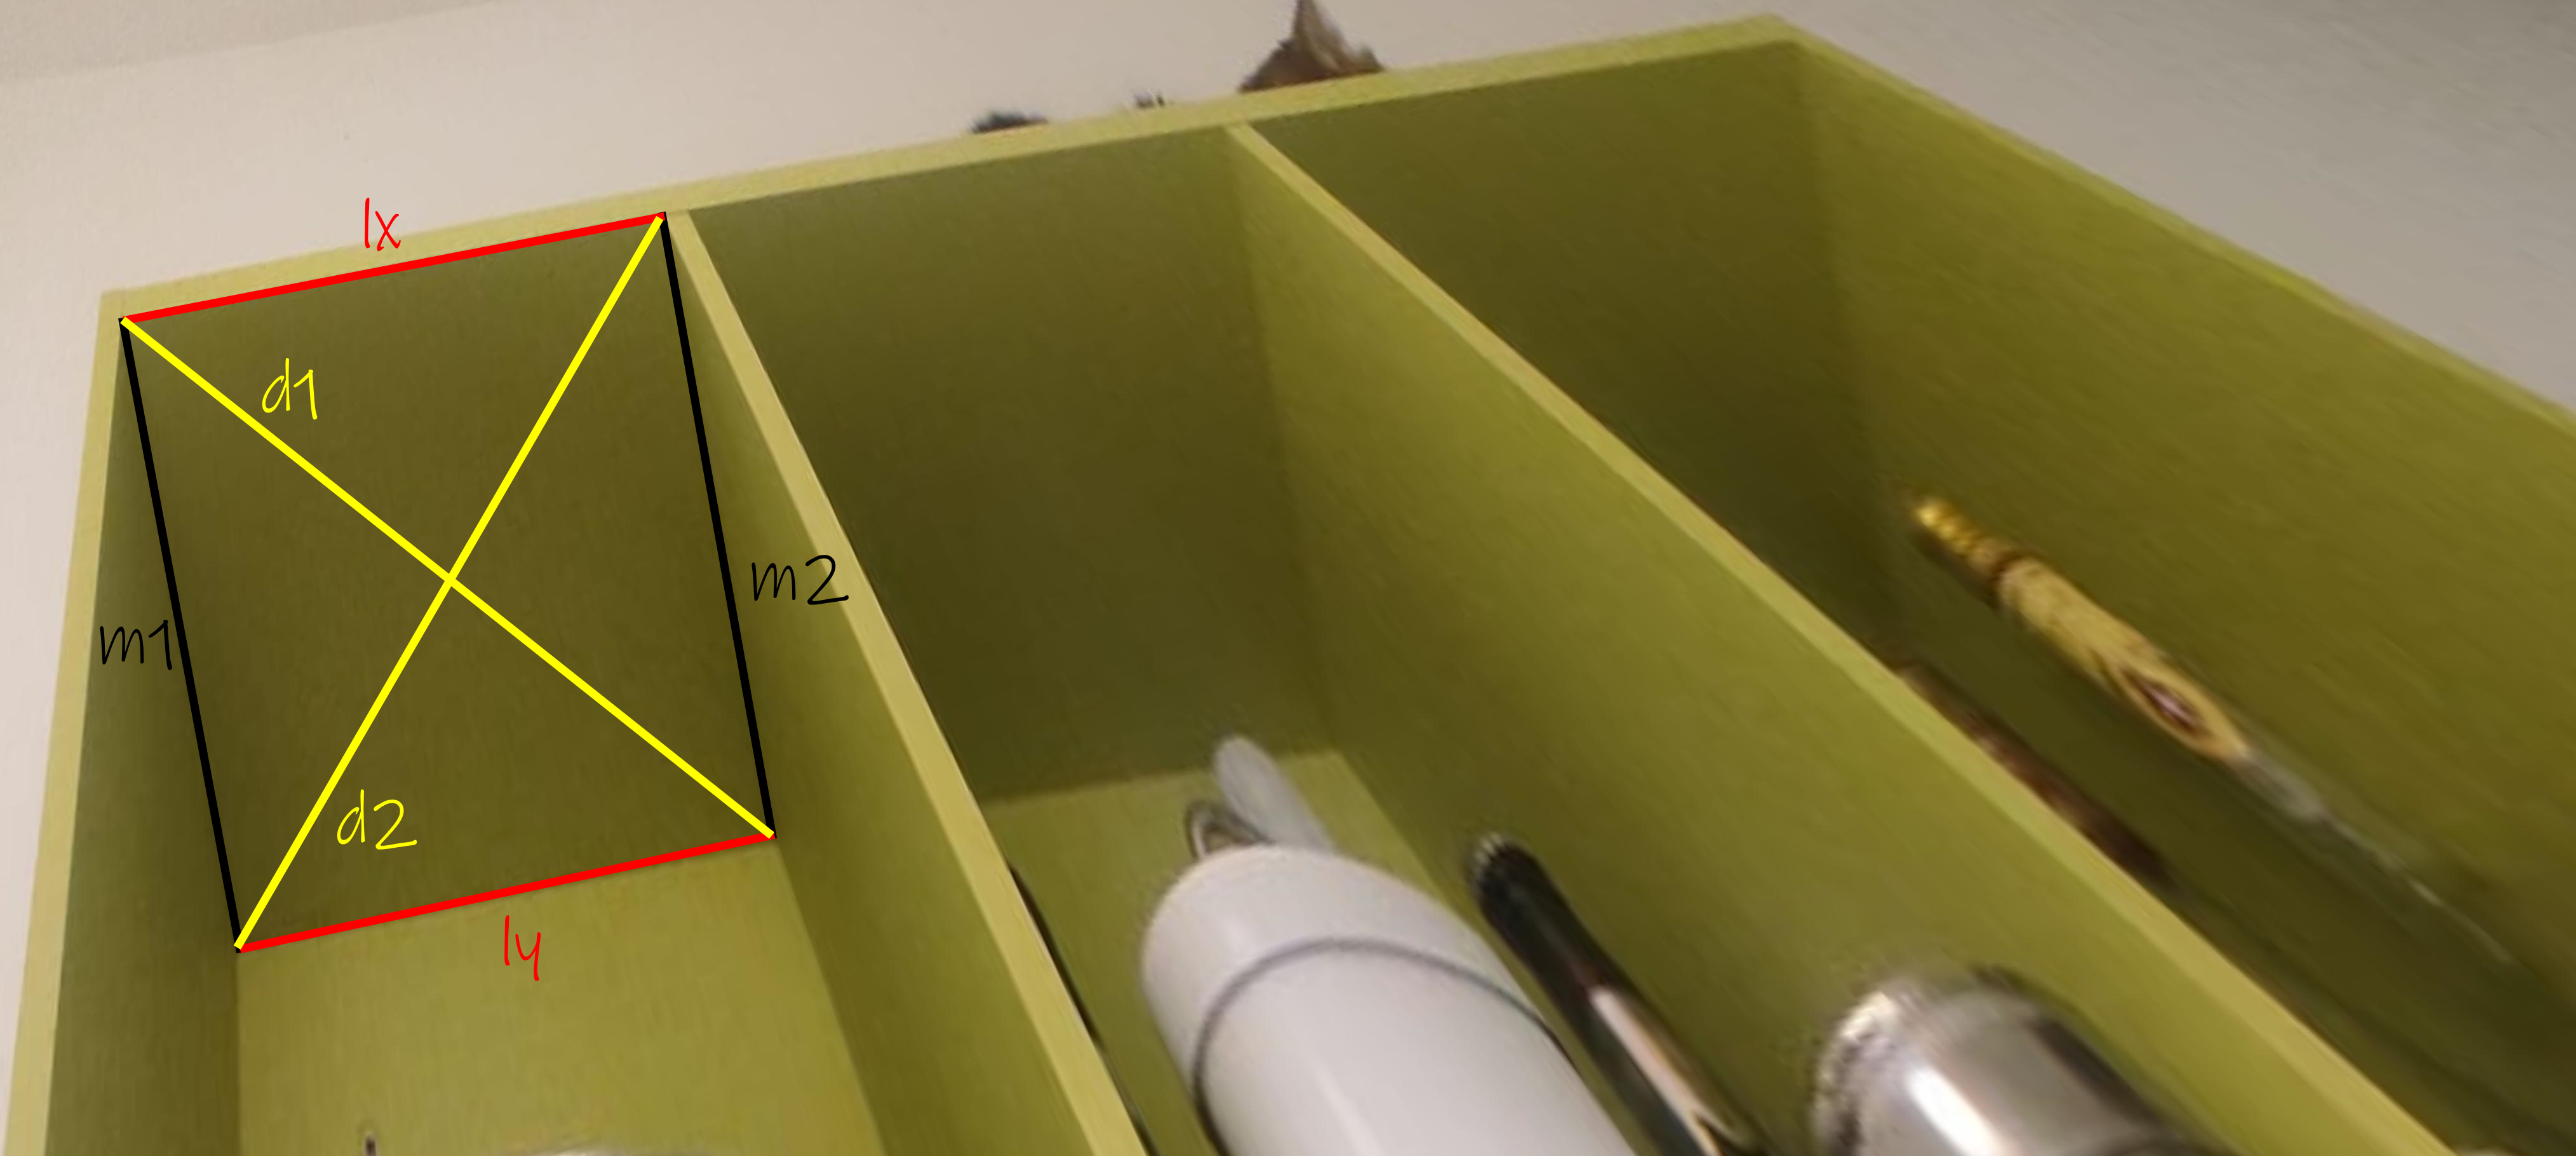
\includegraphics[width=0.5\linewidth]{img/square.png}
    \caption{Square}
    \label{fig:square}
\end{figure}

The angle computed is $\approx 98^{\circ}$, similar to a right one. We can conclude that the figure is a square and finally to conclude that the depth $m$ of the parallelepiped is equal to the length of a single block, about $\frac{1}{3}$ meter, which is a similar value to the one computed previously.

The values are not precisely the same, but they are very similar and we can conclude the depth of the parallelepiped is $\frac{1}{3}$ of the length of it.